%%%%%%%%%%%%%%%%%%%%%%%%%%%%%%%%%%%%%%%%%%%%%%%%
% COPYRIGHT: (C) 2012-2015 FAU FabLab and others
% Bearbeitungen ab 2015-02-20 fallen unter CC-BY-SA 3.0
% Sobald alle Mitautoren zugestimmt haben, steht die komplette Datei unter CC-BY-SA 3.0. Bis dahin ist der Lizenzstatus aller alten Bestandteile ungeklärt.
%%%%%%%%%%%%%%%%%%%%%%%%%%%%%%%%%%%%%%%%%%%%%%%%


\newcommand{\basedir}{fablab-document} % Pfad zur Dokumentenvorlage
\documentclass{\basedir/fablab-document}

\usepackage{amssymb} % Symbole für Knöpfe
\usepackage{subfigure,caption}
\usepackage{eurosym}
\usepackage{tabularx} % Tabellen mit bestimmtem Breitenverhältnis der Spalten
\usepackage{wrapfig} % Textumlauf um Bilder
\usepackage{pdfpages}
\usepackage{booktabs}
\usepackage[colorinlistoftodos,prependcaption]{todonotes}
\presetkeys%
    {todonotes}%
    {inline,backgroundcolor=red}{}
\renewcommand{\texteuro}{\euro}
%\newcommand{\todo}[1]{\textbf{\color{red}{TODO: #1}}}
\newcommand{\pfeil}{\ensuremath{\rightarrow}}
\newcommand{\kommando}[1]{\texttt{#1}}
\newcommand{\tabitem}{~~\llap{\textbullet}~~}
\newcommand{\mcc}[1]{\multicolumn{2}{c}{#1}}
\renewcaptionname{ngerman}{\tablename}{Tab.}

% \linespread{1.2}

\fancyhead[C]{\textbf{\color{red}{TODO: unfertig!}}}
\date{2015}
\author{kontakt@fablab.fau.de}
\title{Grundlagen Drehbank}

\begin{document}

\listoftodos

\tableofcontents

\newpage

\section{Einweisungsstufen}

\begin{itemize}
 \item Ohne eine unterschriebene Grund-Einweisung in diese Regeln darf die Drehbank garnicht benutzt werden, d.\,h. du darfst dann nichts selber an und in der Drehbank tun.
 \item Mit Grund-Einweisung bist du zunächst \enquote{Fahrschüler} und darfst den Auftrag zwar selber vorbereiten (NC-Code laden, Werkstück ein- und ausspannen, Drehbank säubern), \textbf{die Steuerung aber nicht selbstständig bedienen.} 

       Ein Benutzer, der die Drehbank selbstständig benutzen darf, prüft dann, ob dein Auftrag keine gefährlichen Fehler enthält, und führt dann als \enquote{Fahrlehrer} gemeinsam mit dir die Arbeit durch.

 Die Bedienung der Steuersoftware (Verfahren, Antasten, Starten, Fortsetzen nach Pause, \dots) darf dabei nur unter ständiger Aufsicht durch den Experten erfolgen!
 \item Sobald du genug Erfahrung und Routine hast und das entsprechend dokumentiert ist (mehrere Werkstücke selbstständig unter Aufsicht gefertigt, dies über einen größeren Zeitraum verteilt), wird dir die schriftliche Erlaubnis erteilt, den CNC-Betrieb ohne Aufsicht zu benutzen.
 \item  \textbf{Für die Benutzung des Handbetriebs ist eine zusätzliche schriftliche Erlaubnis nötig!} Es gelten dabei weitere Vorschriften, siehe Kapitel \ref{handdrehen}.
\end{itemize}


\newpage
\section{Grundlagen}
\subsection{Begriffserklärung}
\begin{tabular}{p{0.15\textwidth} p{0.8\textwidth}}
Achsen 				& Z längs der Drehachse (nach rechts = positiv), X quer zur Drehachse (nach vorne = positiv) \\
Drehmeißel 		& Komplettes Teil aus Wendeplatte und Wendeplattenhalter. Ist in einem Schnellwechselhalter eingespannt und darf nicht verändert werden. \\
Körnerspitze 	& Die mitlaufende Körnerspitze steckt anstelle des Bohrfutters in der Aufnahme des Reitstocks. Wird zum Gegenspannen von langen Werkstücken verwendet. Festdrehen, bis die Körnerspitze dauerhaft mitdreht, dann nicht mehr fester machen. Genaue Erklärung in Kapitel \ref{handdrehen:gegenspannen}. \\
Nullpunkte 		& Z beim rechten Rand des Werkstücks, X in der Drehmitte \\
Reitstock 		& Gegenlager auf der rechten Seite Hauptachse. Wird verwendet um lange Werkstücke gegenzuspannen. \\
Spannfutter 	& Auf der Hauptspindel befestigt. Haltevorrichtung mit 3 bis 4 Backen, welche das Werkstück aufnehmen und festklemmen. \\
Wendeplatte 	& Das kleine, aus Hartmetall gefertigte Teil, das schließlich das Material zerspant. Brüchig aber sehr hart. Die Kanten können leicht brechen, wenn sie überlastet werden oder Stöße abbekommen. \\
\end{tabular}

\subsection{Zerspanung}
\subsubsection{Was ist Drehen?}
Drehen ist ein zerspanender Prozess bei dem ein fest eingespanntes Werkzeug (Drehmeißel) am sich drehenden Werkstück entlanggeführt wird.
Der Drehmeißel hat eine geometrisch bestimmte Schneide aus Schnellarbeitsstahl (HSS) oder Wendeschneidplatten aus Vollhartmetall (VHM) und wird quer zur Drehrichtung bewegt.
Daraus ergibt sich eine kreisförmige Schnittbewegung und es entstehen rotationssymtrische Werkstücke.
\todo{mehr schreiben}

\newpage
\subsubsection{Drehmeißel}
Ein Drehmeißel besteht aus einem Werkzeugschaft, welcher fest in der Aufnahme befestigt ist. Am vorderen Ende befinden sich die Haupt- und Nebenschneide durch welche das Material
abgetragen wird.
\begin{figure}[ht]
\centering
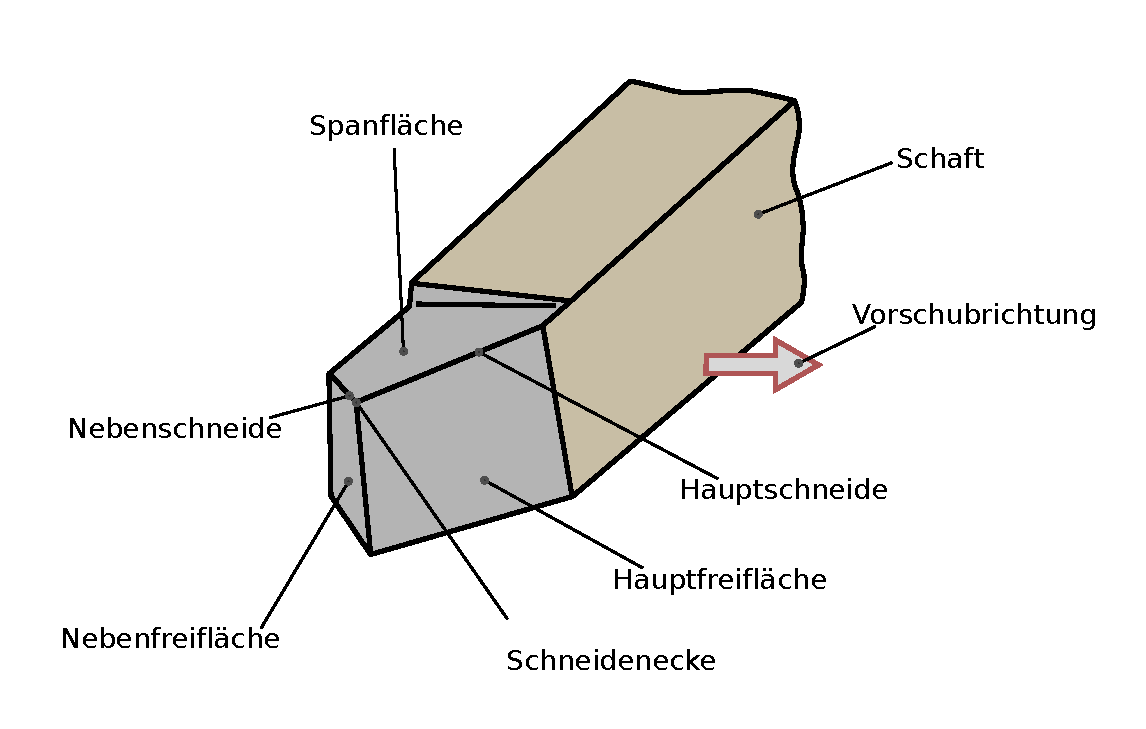
\includegraphics[width = 0.75\linewidth]{img/drehmeissel}
\todo{Autor? Caption? Lizenz?}
\end{figure}

\subsubsection{Spannfutter}

Es gibt zwei verschiedene Spannfutter, eines mit 3 Backen und eines mit 4 Backen. Das Spannfutter wird mit dem entsprechenden Schlüssel an der Seite auf und zu gedreht. Beim Spannen ist das mit \emph{0} markierte Loch zu verwenden.

Es gibt im Grunde keine feste Regel nach der das Futter gewählt werden kann, jedoch gibt es einige Erfahrungswerte:
\begin{itemize} 
\item Rundmaterial im Dreibackenfutter spannen
\item Beim Drehen von Passungen kann das Vierbackenfutter von Vorteil sein (Stichwort \enquote{Dreibogengleichdick})
\item 6-Kant-Material ausschließlich im Dreibackenfutter
\item Objekte mit quadratischem Querschnitt ausschließlich im Vierbackenfutter
\end{itemize}

\subsubsection{Spannfutterwechsel}

Achtung das Spannfutter ist schwer! Lass dir am Besten von jemandem helfen. Achte unbedingt auf Sauberkeit!
\begin{itemize}
\item Maul- und Imbusschlüsselsatz holen
\item Abdeckhaube wegklappen
\item Am Besten etwas unterlegen, damit es nicht herunterfällt
\item Schrauben auf der Rückseite des Futters lösen und dabei festhalten 
\item Nach dem Lösen vorsichtig herausnehmen, ggf. vorsichtig mit dem Schonhammer nachhelfen
\item Hinten am Futter befindet sich ein Adapter für die Aufnahme, dieser muss nun mit einem Innensechskant abgeschraubt werden
\item Den Adapter auf das andere Futter montieren
\item Das neue Futter wieder vorsichtig einsetzen und beim Festschrauben darauf achten, dass es nicht verkantet
\item Das ausgebaute Futter vor dem Einlagern säubern und ölen
\end{itemize}

\subsubsection{Spannbacken}

Es gibt Innen- und Außenspannbacken.
Innenspannbacken werden zum Spannen von Innenradien wie z.\,B. Bohrungen verwendet oder
zum Spannen auf Außenflächen bei kleinen Außendurchmessern.\todo{Ist der vorherige Satz korrekt?}
Außenspannbacken kommen hingegen beim Spannen auf Außenflächen zum Einsatz.
Wichtig: Sechskantmaterial immer mit den Innenbacken spannen.

\todo{Bilder}

\subsubsection{Spannbackenwechsel}
\label{zerspanung:spannbackenwechsel}
Achte \emph{unbedingt} auf Sauberkeit!
 
Die Spannbacken befinden sich in der Schublade unter der Drehbank.
Um die alten Spannbacken zu entfernen muss man diese mit dem Spannfutterschlüssel herausdrehen.
Die Spannbacke mit der Nummer 3 löst sich zuerst, danach die Nummer 2 und 1.
Achte dabei darauf, dass die Spannbacken nicht herausfallen.

Das Einsetzen der neuen Spannbacken beginnt mit der Nummer 1.
Unbedingt darauf achten, dass die Spannbacke Nummer 1 auch an der Postion 1 des Spannfutters eingesetzt wird!
Achte darauf keinen Schmutz oder Späne ins Futter zu bringen.

Das Prinzip der Spannbackenbefestigung ist eine Spirale, die in die Nuten der Spannbacken greift.
Drehe solange den Spannfutterschlüssel, bis der Beginn der Spirale bei Spannbacken 1 zu sehen ist.
Dann drehe ein kleines Stück zurück und schiebe die Spannbacke bis zum Anschlag in die Nut und drehe mit dem Spannfutterschlüssel ein wenig weiter.
Das Vorgehen wiederholt man bei den Spannbacken 2 und 3.

Zum Ende das Futter einmal vollständig zu drehen.
Wenn nun die Spannbacken sauber schließen ist alles richtig gemacht.
Wenn eine Spannbacke jedoch zu früh oder zu spät in der Mitte ankommt, wurde diese falsch eingesetzt.
In diesem Fall müssen alle Spannbacken wieder ausgebaut und die Prozedur komplett wiederholt werden.

Die ausgebauten Spannbacken säubern, ölen und wieder aufräumen.

\subsubsection{Kühlschmierstoff}

Das Kühlmittel besteht aus einer Öl-Wasser-Emulsion.
Die Aufgabe des Kühlschmierstoffes (KSS) besteht darin den Schneidvorgang zu kühlen (Wasser) und zu schmieren (Öl).
Aufgrund der Zusätze und der entfettenden Wirkung des Emulgators sollte der Hautkontakt vermieden werden.
Bei Augenkontakt sofort mit reichlich Wasser ausspülen und gelegentlich die oberen und unteren Augenlieder anheben.
Anschließend ist ein Augenarzt aufzusuchen.

\subsubsection{Drehbank}
\todo{Bild mit Beschreibung: Bild Philipp, Michael}
Unsere Drehbank besteht aus Hauptspindel mit Schutzhaube, Reitstock, Werkzeughalter, Kühlmittelpumpe, CNC-Steuerung und Einhausung mit Schutzhaube
\begin{figure}[ht]
\centering
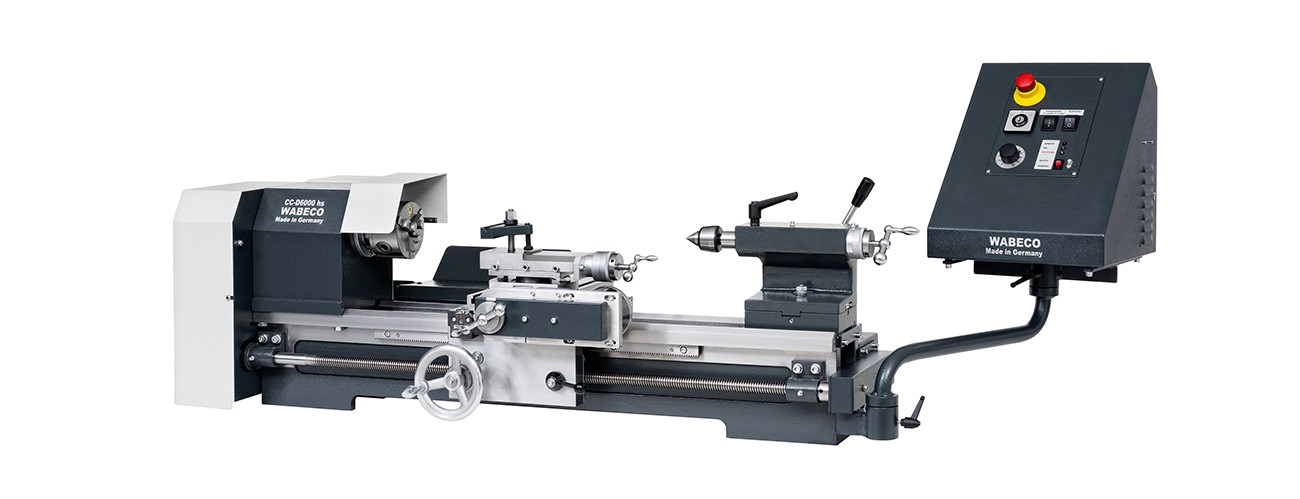
\includegraphics[width = 0.9\linewidth]{img/drehbank} \\
\todo{durch besseres Bild ersetzen}
\end{figure}


\subsubsection{Drehprozess}
\begin{tabular}{lll}
    Schnittgeschw. in $\frac{m}{min}$ 					& $v_c = \pi \cdot d \cdot n $ 			& Geschwindigkeit mit der das Material auf den Drehmeißel trifft 	\\ 
																								&																		& Material- und geometrieabhängiger Wert siehe \ref{Schnittwerte} \\ \addlinespace
		Drehzahl in $\frac{1}{min}$ 								& $ n = \frac{v_c}{\pi \cdot d} $		& Drehzahl der Hauptspindel, ergibt sich aus $V_c$								\\ \addlinespace
		Vorschub in $mm$ 														& $ f_z $  													& Materialstärke welche pro Umdrehung abgetragen wird 						\\
																								&																		& Material- und geometrieabhängiger Wert siehe \ref{Schnittwerte} \\ \addlinespace
		Vorschubgeschw. in $\frac{mm}{min}$ 				& $ v_f = n \cdot f_z $ 						& Geschwindigkeit mit der der Drehmeißel verfährt			 						\\ \addlinespace
		Zustellung in $mm$ 													& $ h  $  													& Materialstärke welche auf einmal vom Radius weggenommen wird		\\
																								&																		& Material- und prozessabhängiger Wert siehe \ref{Schnittwerte} 	\\ \addlinespace
\end{tabular}

\begin{figure}[ht]
\centering
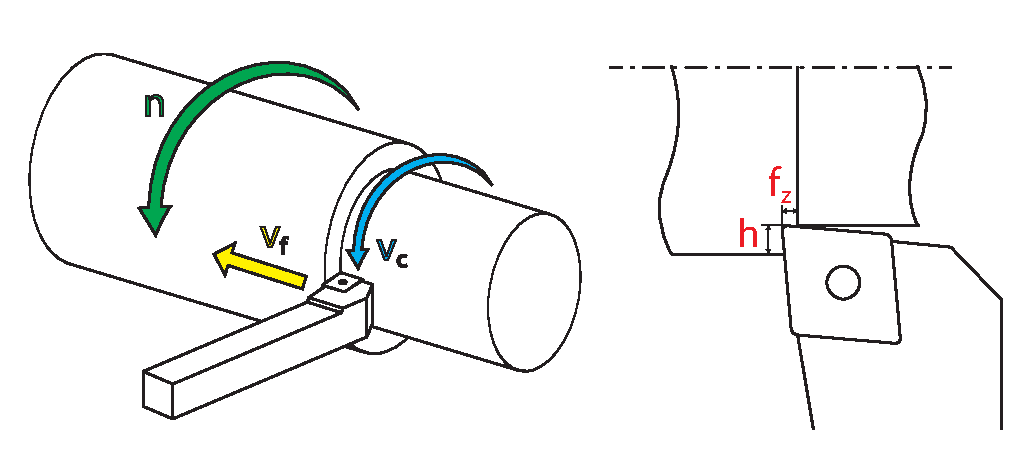
\includegraphics[width = 0.9\linewidth]{img/drehprozess}
\todo{Autor? Caption? Lizenz?}
\end{figure}


\subsubsection{Spanformen}
Die Spanbildung bzw. Spanform ist sehr wichtig für die erreichbare Oberflächengüte und hängt sowohl vom Material, als auch von den Prozessparametern ab. \\[1em]
\begin{tabular}{ll}
    Fließspan		& \tabitem kontinuierliche, fließende Spanbildung (Achtung! Verhedderungsgefahr)													\\ 
								&	\tabitem großer Spanwinkel, hohe Schnittgeschwindigkeit, $v_c > 80 \frac{m}{min} $											\\
								&	\tabitem Spanen gut plastisch verformbarer Werkstoffe, z.\,B. Aluminium																		\\
								&	\tabitem hohe Oberflächengüte																																						\\ \addlinespace
    Scherspan		& \tabitem lamellenförmig abgetrennte Spannteilchen, verschweißen wieder in der Scherzone									\\ 
								&	\tabitem mittlere Spanwinkel und Schnittgeschwindigkeit, $20 \frac{m}{min} < v_c < 80 \frac{m}{min} $		\\
								&	\tabitem Spanen zäherer Werkstoffe, z.\,B. Stahl mittlerer Festigkeit 																		\\
								&	\tabitem mittlere Oberflächengüte																																				\\ \addlinespace
    Reißspan		& \tabitem Herausreißen einzelner Spanteile aus dem Werkstoff																							\\ 
								&	\tabitem kleiner Spanwinkel, niedrige Schnittgeschwindigkeit, $v_c < 20 \frac{m}{min} $									\\
								&	\tabitem Spanen spröder Werkstoffe, z.\,B. Gusseisen, Hartguss, Kupfer-Zink-Legierungen, Messing					\\
								&	\tabitem raue Werkstückoberfläche																																				\\ \addlinespace
\end{tabular}
\begin{figure}[ht]
\centering
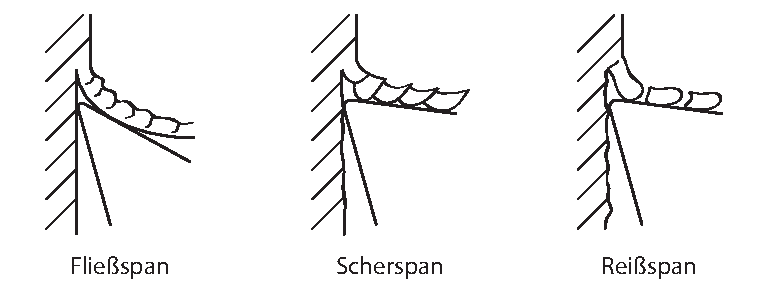
\includegraphics[width = \linewidth]{img/spanformen}
\todo{Autor? Caption? Lizenz?}
\end{figure}

\subsubsection{Schnittwerte}
\label{Schnittwerte}
\todo{Hinweis, woher Werte kommen. Hinweis, dass nicht ideal}
Der Vorschub ist in den Datenblättern meist als spezifischer Vorschub angegeben (mm pro Umdrehung) und muss entsprechend mit der Drehzahl multipliziert werden.
In der Praxis nimmt man die ungefähre Größenordnung aus der Tabelle und probiert.

Zu niedriger Vorschub führt dazu, dass zu wenig Span abgenommen wird und das Werkstück eher gerieben als zerspant wird.
Das setzt das Werkzeug zu und verschlechtert die Schneide.
Zu hoher Vorschub hingegen belastet Werkzeug und Maschine unnötig,
führt zu erhöhtem Verschleiß und kann die Spindel überlasten, wodurch die Drehzahl einbricht.

Die Zustellung ist immer als Absolutwert angegeben.
Bei der Zustellung sind die Auswirkungen ähnlich wie beim Vorschub.

Bei zu großer Zustellung können Stücke aus dem Material ausreißen oder das Werkstück aus dem Futter
springen und den Bediener schwer verletzen!

Dabei gilt, dass der Vorschub beim sogenannten Schruppen höher ist als beim Schlichten.
Schruppen dient in erster Linie dem Abtrag von Material und erzeugt in der Regel eine rauhe Oberfläche mit Riefen.
Schlichten hingegen ist die finale Bearbeitung auf das endgültige Maß in meist einem Durchgang.
Die Oberfläche wird dabei wesentlich feiner. 

\begin{table}
\setlength{\tabcolsep}{0.5em}

\todo{Autor? Caption? Lizenz?}
\begin{tabular}{rcccccc}
  \textbf{Werkstoff}  & \mcc{$\mathbf{v_c} \textrm{ in } \frac{m}{min} $} & \mcc{$\mathbf{f_z} \textrm{ in } mm$} & \mcc{$\mathbf{h_{max}} \textrm{ in } mm$} \\ \addlinespace \toprule
															& Schruppen 	& Schlichten 	& Schruppen 	& Schlichten 	& Schruppen 	& Schlichten		\\ \toprule
  unleg. Stahl (0,15\% C)			& 370 	& 420  	& 0.17 	& 0.12	& 3.5 	& 1.0 	\\
  unleg. Stahl (0,45\% C)			& 280 	& 315  	& 0.20 	& 0.15	& 3.5 	& 1.0 	\\
  unleg. Stahl (0,55\% C)			& 255 	& 295  	& 0.20 	& 0.15	& 3.5 	& 1.0 	\\
	leg. Stahl									& 345 	& 380  	& 0.17 	& 0.12	& 3.5 	& 1.0 	\\
	leg. Stahl (Cr-Mo)					& 255 	& 295  	& 0.20 	& 0.15	& 3.5 	& 1.0 	\\	
	leg. Stahl (Ni-Cr-Mo)				& 250 	& 285  	& 0.20 	& 0.15	& 3.5 	& 1.0 	\\
	Wälzlagerstahl							& 255 	& 295  	& 0.20 	& 0.15	& 3.5 	& 1.0 	\\
	unleg. Werkzeugstahl				& 255 	& 295  	& 0.20 	& 0.15	& 3.5 	& 1.0 	\\	
	leg. Werkzeugstahl					& 250 	& 285  	& 0.20 	& 0.15	& 3.5 	& 1.0 	\\	
	Schnellarbeitsstahl					& 145 	& 210  	& 0.15 	& 0.10	& 3.5 	& 1.0 	\\	
	Kaltarbeitsstahl						& 195 	& 225  	& 0.18 	& 0.14	& 3.5 	& 1.0 	\\	
	gehärteter Stahl ($<$40HRC)	& 120 	& 120  	& 0.12 	& 0.10	& 3.5 	& 1.0 	\\	
	hochleg. Stahl	(mart./fer.)& 195 	& 270  	& 0.17 	& 0.12	& 3.5 	& 1.0 	\\
	hochleg. Stahl	(aust.)			& 160 	& 220  	& 0.17 	& 0.12	& 3.5 	& 1.0 	\\
	Superlegierung (Ni)					& 50	 	& 60  	& 0.15 	& 0.10	& 3.5 	& 1.0 	\\
	Titan												& 80	 	& 100  	& 0.15 	& 0.10	& 3.5 	& 1.0 	\\
	Grauguss										& 380	 	& 400  	& 0.25 	& 0.18	& 3.5 	& 1.0 	\\
	Stahlguss										& 305	 	& 320  	& 0.20 	& 0.15	& 3.5 	& 1.0 	\\
	Aluminium	($<$12\% Si)			& 500	 	& 500  	& 0.25 	& 0.15	& 3.5 	& 1.0 	\\
	Aluminium	($>$12\% Si)			& 150	 	& 150  	& 0.22 	& 0.13	& 3.5 	& 1.0 	\\
	Kupfer											& 400	 	& 400  	& 0.20 	& 0.15	& 3.5 	& 1.0 	\\
	Messing											& 400	 	& 400  	& 0.20 	& 0.15	& 3.5 	& 1.0 	\\
	Acryl												& 200	 	& 300 	& 0.50 	& 0.10	& 6.0 	& 1.0 	\\
	Kunsstoff										& 500	 	& 800 	& 0.40 	& 0.10	& 6.0 	& 1.0 	\\
	Hartholz										& 60	 	& 90  	& 0.30 	& 0.15	& 6.0 	& 1.0 	\\
	Weichholz										& 70	 	& 110  	& 0.30 	& 0.15	& 6.0 	& 1.0 	\\
\end{tabular}

\end{table}

\newpage
\section{Sicherheit und Verhaltensregeln}
\subsection{Schutzmaßnahmen und Verhaltensregeln}
Die hier beschriebenen Abläufe müssen unbedingt eingehalten werden.
Bei Unklarheiten nachfragen!
\begin{itemize}
\item \textbf{Die Maschine darf niemals von zwei oder mehr Personen gleichzeitig bedient werden. Massive Gefährdung möglich!}
\item Nur der Maschinenbediener und maximal eine weitere eingewiesene Person dürfen sich im Sicherheitsbereich aufhalten.\\
\todo{Zeichnung vom Sicherheitsbereich}
\item \textbf{Im Sicherheitsbereich ist immer eine Schutzbrille zu tragen!}
\item Die Regeln für den Sicherheitsbereich gelten, sobald an der Maschine gearbeitet wird bzw. sobald die Absperrbänder gespannt wurden.
\item Grundlegende Verhaltensregeln stehen in der Betriebsanweisung (blaue Seite am Ende dieses Abschnitts).
\item Besondere Vorkommnisse sind unverzüglich dem Maschinenverantwortlichen (siehe Schild auf der Steuerung) zu melden.\\
Bei Problemen ist eine Störungsmeldung (Zettel) an der Maschine anzubringen und, wenn die Sicherheit beeinträchtigt ist, die Maschine außer Betrieb zu nehmen.

\item Vor Beginn der Arbeit:
\begin{itemize}
\item Gesamtzustand der Maschine überprüfen
\item Die Drehbank darf nur dann benutzt werden, wenn die beiden Absperrbänder gespannt wurden. Es dürfen sich dann nur in die Drehbank eingewiesene Personen in diesem Bereich befinden!
\item Lange Haare durch Mütze, Haarnetz o.\,ä. verdecken; einfaches Zusammenbinden ist nicht ausreichend! Mützen sind selbst mitzubringen, können aber auch gestellt werden.
\end{itemize}

 \item Die Schutzhaube darf nur offen sein, solange die Spindel steht. (Dies gilt nicht für den Handbetrieb.) Nachlaufdauer!  % wird zwar teils durch den Schalter erzwungen, aber trotzdem Nachlaufgefahr.
 \item Spannschlüssel \textbf{nie} im Futter stecken lassen. % \\ Der Spannschlüssel darf nicht manipuliert sein, die Sicherheits-Feder muss aufgesteckt bleiben. - Nicht zwingend Notwendig nach BGI 5003 2.5.1.2
 \item Zum Reinigen oder Warten ist die Maschine auszuschalten!
 \item Metallspäne können sehr scharf und heiß sein (besonders bei Stahl und Edelstahl). Späne dürfen nicht von Hand beseitigt werden, Spänehaken, Zange, Pinsel, Wischer oder Staubsauger verwenden. % per Hand nicht zulässig nach BGI 5003 2.5.

 \item Beim Hantieren in der Drehbank:
\begin{itemize}
 \item Anleitung exakt beachten. Wenn du nicht ganz genau weißt was du tust, nachfragen!
 \item Schutzhaube nur öffnen, wenn die Spindel steht (Nachlauf abwarten!). Die Schutzhabe ist kein zulässiger Not-Aus-Schalter!
\item Im Notfall die Maschine durch Drücken des Not-Aus-Schalters stoppen.
\item Im CNC-Modus darf keine der Kurbeln von Hand bedient werden! Verletzungsgefahr! Falls doch geschehen, hat die Maschine Schritte auf der jeweiligen Achse verloren. Das Resultat ist eine verlorene Maschinenreferenzierung (muss wiederholt werden) und ein verschobener Werkstücknullpunkt (wird durch Maschinenreferenzierung wieder behoben, trotzdem kontrollieren!).
\end{itemize}
\item Nach der Arbeit muss die Maschine gemäß der Anleitung gesäubert und das Werkzeug überprüft werden, ggf. verschüttetes KSS auf dem Boden beseitigen (Rutschgefahr!)
%\item für besondere Bearbeitungen sind noch weitere Regeln zu beachten. % allgemeiner satz, bitte noch gescheit formulieren.

\end{itemize}
\subsection{Sicherheitseinrichtungen}
Die Maschine ist mit mehreren Sicherheitseinrichtungen und -funktionen ausgestattet:
\begin{itemize}
	\item Not-Aus-Schalter auf dem Handteil über der Maschine: Drücken führt zum sofortigen Stromlosschalten der Antriebe. Achtung: Hauptspindel läuft nach.
	\item Not-Aus-Rücksetztaster am Schaltschrank: Nach Not-Aus oder Stromausfall sicherstellen, dass die Spindel ausgeschaltet ist (Hand-Drehrichtungs-Schalter auf 0), dann mit diesem Schalter die Maschine wieder anschalten.
	\item Hauptschalter am Schaltschrank: Ist nach Ende der Benutzung auszuschalten.
	\item Spannfutter-Abdeckung: Ist der weißlackierte Blechdeckel über dem Spannfutter geöffnet, ist ein Anlaufen der Spindel unmöglich.
	\item Einhausung: Die Haube ist mit einem Not-Aus-Kontakt ausgestattet, welcher bei laufendem CNC-Programm eine Abschaltung auslöst. Achtung: Bei Handbetrieb deaktiviert!
	\item Über Tastatureingabe ist nur ein Abbrechen oder Anhalten des Jobs möglich. Dies ersetzt keinen Not-Aus!
\end{itemize}

\clearpage
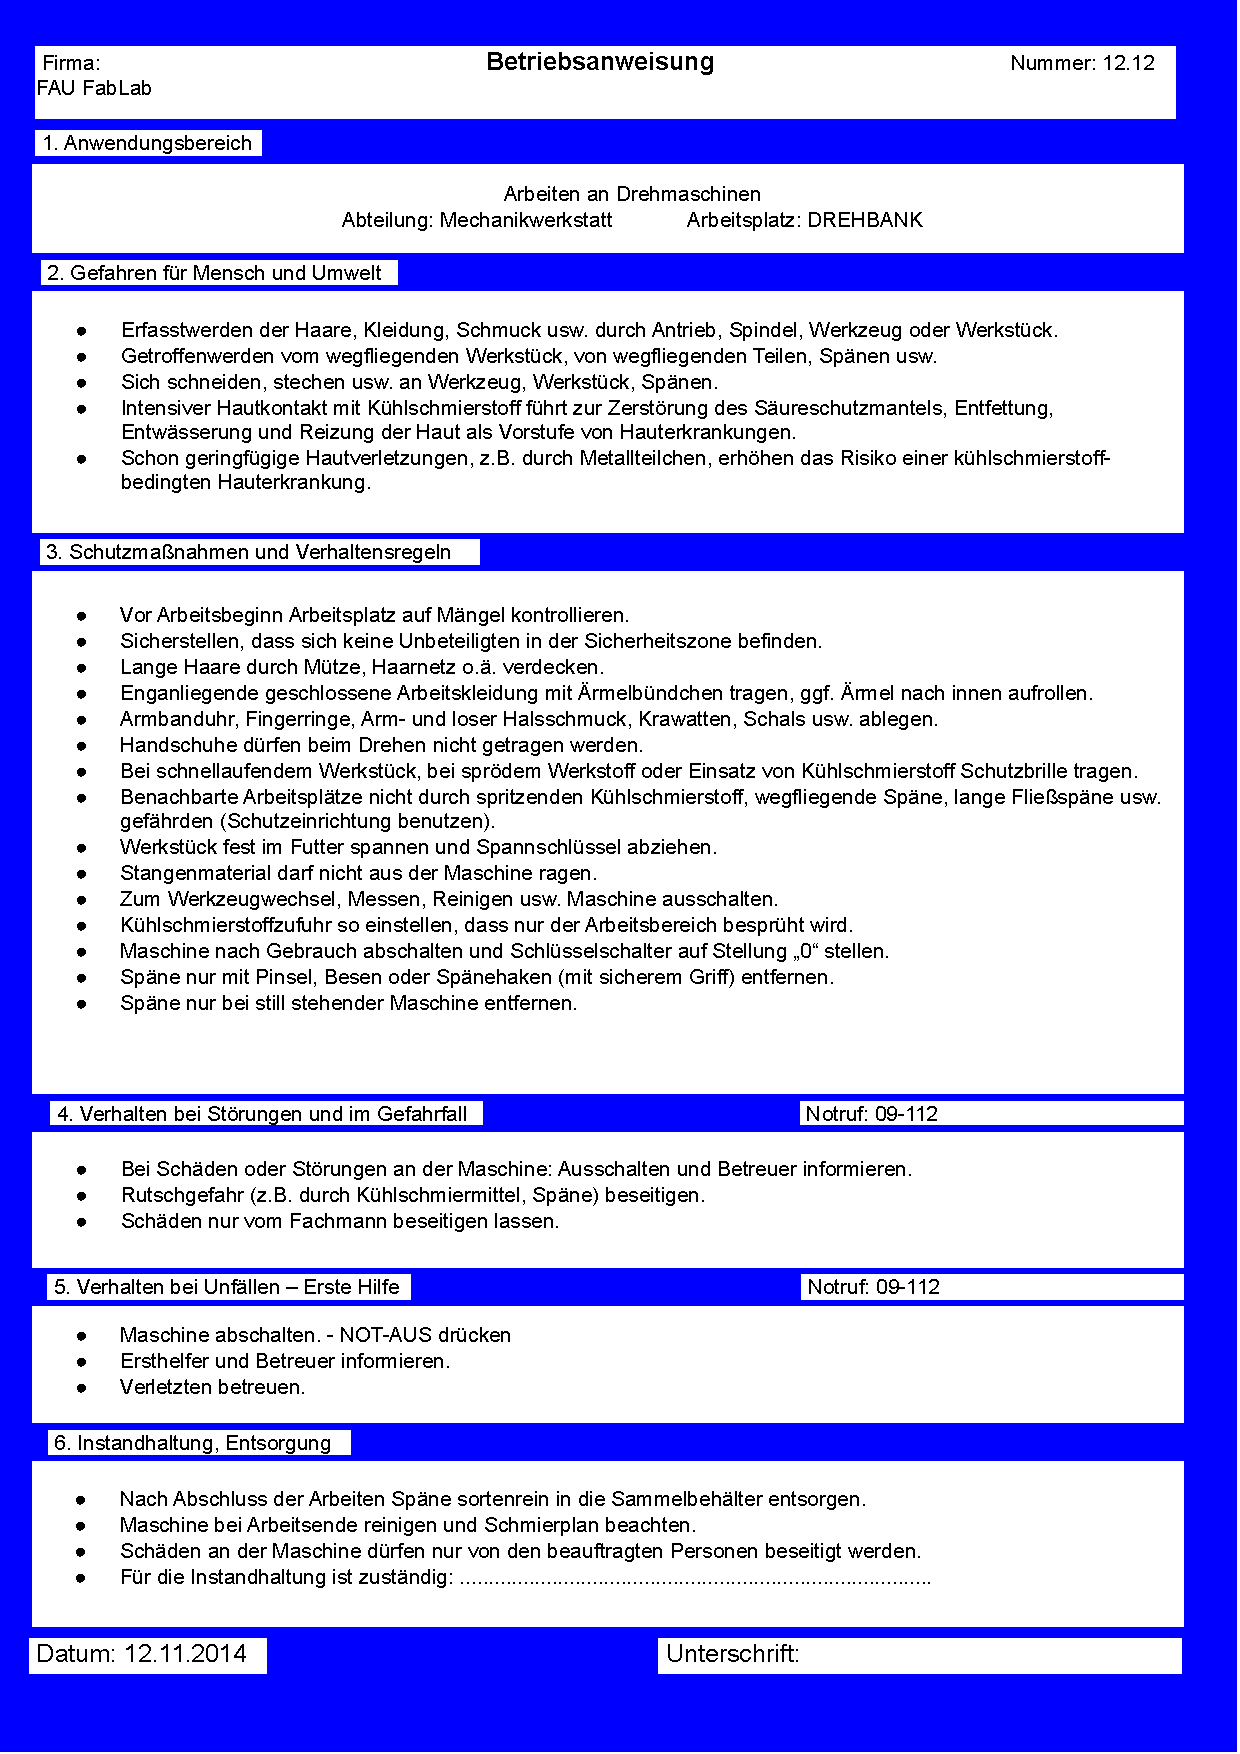
\includepdf[pages=1]{Drehmaschinen.pdf}
\newpage
\section{Vorbereitende Aufgaben}
\subsection{Rohmaterial einspannen}

Achte vor dem Einspannen darauf das passende Futter zu verwenden.
Zum Wechseln siehe Kapitel \ref{zerspanung:spannbackenwechsel}.

Öffne die Spannbacken vor dem Einsetzen auf einen adäquaten Durchmesser und setze das Rohmaterial
plan zu den Auflageflächen der Spannbacken ein.
Achte beim Festziehen darauf, dass das Material eine möglichst geringe Unwucht hat.
Das Werkstück darf in keinem Fall wackeln oder rutschen können.
Bei hohen Drehzahlen muss das Werkstück unbedingt fest gespannt werden!
(Der Fliehkrafteinfluss verringert die Spannkraft.)
Außerdem sollte es möglichst weit in das Spannfutter gesteckt werden.
Achte dabei auf einen Sicherheitsabstand von 1\,mm zwischen Spannfutter und Drehmeißel.

Lange oder schlanke Werkstücke müssen mit dem Reitstock gegengespannt werden,
wie im Kapitel \ref{handdrehen:gegenspannen} beschrieben.

\subsection{Werkzeug einsetzen} %Eventuell Praxsistipps anhängen
Achte vor dem Einsetzen darauf, die richtige Wendeplatte zu verwenden. Zum Wechseln siehe \todo{Abhandlung über den Wechsel von Wendescheidplatten}.

Am Schnellwechselhalter wir der Hebel so gestellt, dass die Halteklammern maximal geöffnet sind.
Das eingespannte Werkzeug sollte sich jetzt leicht nach oben abziehen lassen.
Das neue Werkzeug wird nach dem gleichen Prinzip eingesetzt und mit dem Hebel handfest gespannt.

Achte darauf, dass der Schnellwechselhalter nicht verdreht ist.

\subsection{Kühlung einrichten}

Bei der Bearbeitung von Metall ist KSS zwingend nötig, bei Kunststoff nicht.
Im CNC-Betrieb ist die Kühlung voll aufzudrehen und im Handbetrieb entsprechend zu reduzieren,
um ein übermäßiges Herausspritzen des KSS zu verhindern.
Der Strom ist dabei auf die Schneide der Schneidplatte auszurichten.

Im Handbetrieb kann alternativ, besonders zum Abstechen, mit einer kleinen Ölflasche geschmiert werden. 

\newpage
\section{Handdrehen}
\label{handdrehen}
\subsection{Skalen}

Die Skalen an den beiden Handrädern können über Drehen des Skalenrings auf \emph{0} \enquote{genullt} werden.
Dabei das Handrad festhalten.
Dabei gilt folgende Skalierung:
\begin{itemize}
\item Z-Achse: Die aufgeprägten Zahlen entsprechen 1/10\,mm 
\item X-Achse: Die aufgeprägten Zahlen entsprechen 1\,mm Durchmesser
\item Oberschlitten: Die aufgeprägten Zahlen entsprechen 1/10\,mm 
\item Reitstock: Skala auf der Reitstockpinole oder Drehrad, dabei entsprechen die aufgeprägten Zahlen 1/2\,mm
\end{itemize}

\todo{Bild mit Achsenbezeichnung}

\subsection{Zentrierbohrung}
\label{handdrehen:zentrierbohrung}
Das Setzen einer Zentrierbohrung ist wichtig, um das Verlaufen des Bohrers beim Bohren zu verhindern
und das Gegenspannen des Werkstückes mit einer mitlaufenden Körnerspitze zu ermöglichen.
Bevor überhaupt eine Zentrierbohrung gesetzt werden kann ist die Fläche vorher wie in
Abschnitt \ref{handdrehen:Plandrehen} beschrieben plan zu drehen!

\todo{Zeichung von Bohrtiefe, wie tief muss ich mit dem Werkzeug eintauchen, untersch. Tiefen Bohrung, Zentrieren}

Für die Zentrierbohrung ist der Zentrierbohrer ohne Klebeband zu verwenden.
Unbenutzte, neue Zentrierbohrer sind mit Klebeband markiert.

Falls das Bohrfutter nicht im Reitstock eingespannt ist, muss zunächst das dort montierte Werkzeug entfernt werden.
Dazu wird die Kurbel des Reitstockes soweit zurück gedreht, bis der  Kegel aus dem Reitstock gedrückt wird.
Dies kann etwas (aber nicht allzu viel) Kraft benötigen.
Manchmal hilft es auch ein wenig \enquote{Schwung} zu holen.

In die freie Kegelaufnahme des Reitstockes (sogenannte Reitstockpinole) wird dann das Bohrfutter eingeschoben.
Dazu muss die Pinole mindestens auf 15\,mm ausgefahren sein.
Unbedingt den sicheren Sitz des Werkzeuges prüfen!

\textbf{Unbedingt darauf achten, dass hierbei keinerlei Späne auf dem Bohrfutterkegel oder in der Reitstockaufnahme sind! Falls das Bohrfutter oder die mitlaufende Körnerspitze mit einem Span geklemmt wird, ist es sehr wahrscheinlich, dass sich weder das Futter noch die Spitze jemals wieder demontieren lassen ohne etwas ernsthaft zu beschädigen!}

Vorgehen:
\begin{itemize}
\item Zentrierbohrer einspannen
\item Reitstock bis an Material heran fahren und festklemmen
\item Richtige Drehzahl einstellen
\item Mit guter Handkraft bohren und immer wieder mit Öl schmieren!
\item Richtige Senkungstiefe beachten
\item Wenn die nötige Tiefe erreicht ist, Reitstockpinole zurück kurbeln

\end{itemize}

\subsection{Bohren}

Um das Verlaufen des Bohrers zu vermeiden ist es zunächst notwendig eine Zentrierbohrung wie im Kapitel \ref{handdrehen:zentrierbohrung} beschrieben anzubringen.
Anschließend bringt man das Bohrfutter an der Reitstockspindel an und wählt den passenden Bohrer aus.
Verwende hierfür unbedingt die Bohrer, die sich in der Schublade unter der Drehbank befinden.

Positioniere den Bohrer kurz vor dem Werkstück und wähle die passende Drehzahl aus der Drehzahltabelle an der Drehbank aus.
Danach kann durch Zustellung mit der Reitstockpinole gebohrt werden.
Dabei gilt wie bei jedem Bohrvorgang: Mit guter Handkraft bohren!
Ansonsten wird der Bohrer übermäßig verschlissen und die Qualität der Bohrung nimmt ab.

\subsection{Außendrehen} 

Das Außendrehen findet in der Regel in mehreren Bahnen mit dem richtigen Vorschub und Zustellung statt.
Hierbei wird grundsätzlich zum Futter hingearbeitet.
Es ist darauf zu achten auf keinen Fall mit dem Werkzeug ins Futter zu fahren, da ein solcher Crash Werkzeug und Maschine ernsthaft beschädigen und den Bediener schwer verletzen kann.
Am Ende ist in Richtung des Durchmessers vom Werkstück wegzufahren, bevor in Z-Richtung zum Beginn einer neuen Bahn gefahren wird.

\subsection{Innendrehen}

Das Innendrehen funktioniert im Grunde wie das Außendrehen. Es gibt jedoch trotzdem einige Besonderheiten:
\begin{itemize}
\item Anders als beim Außendrehen sieht man sein Werkzeug nur schlecht. Achte unbedingt darauf keine Kollision zu fahren.\\
\textbf{Nicht in die laufende Maschine beugen und versuchen so das Werkzeug zu sehen!}
\item Die Zustellung erfolgt beim Innendrehen in negativer Richtung, d.\,h. um 1\,mm abzunehmen ist mit dem Handrad 1\,mm zurückzufahren.
\end{itemize}

\subsection{Fasen}

Für das Anbringen von 45$^\circ$ Fasen gibt es ein spezielles Werkzeug, einen sogenannten Fasenmeißel.
Das Werkzeug ist gut an seiner blauen Lackierung und der breiten Schneide zu erkennen.
Den Fasenmeißel spannt man senkrecht zum Werkstück ein, sodass die Schneide 45$^\circ$ zum Werkstück zeigt.
Danach kann an das Werkstück herangefahren werden und eine Fase angebracht werden.
Wenn sehr viele Fasen angebracht werden müssen, empfiehlt es sich nicht immer auf der selben Stelle der Schneide zu arbeiten.
Dies soll verhindern, dass die Schneide ungleichmäßig abgenutzt wird.

Für andere Winkel kann der Werkzeughalter mit dem Fasenmeißel auch verdreht in das Schnellspannfutter eingesetzt werden.

\subsection{Plandrehen}
\label{handdrehen:Plandrehen}

Um eine Fläche an einem Werkstück plan zu drehen, fährt man das Werkzeug bis kurz vor die zu planende Fläche. Nun kommt es darauf an, ob die zu planende Fläche als Referenzfläche oder als Fläche für eine Zentrierbohrung vorbereitet werden soll. 

Im Falle einer Referenzfläche muss zunächst der Nullpunkt in axialer Richtung gesucht werden.
Dazu bewegt man das Werkzeug soweit in radialer Richtung bis die Schneideplattenspitze sich in radialer Richtung innerhalb des Werkstückes befindet.
Nach dem Starten der Spindel wird das Werkzeug vorsichtig in axialer Richtung auf das Werkstück zu bewegt.
Sobald die Schneideplatte beginnt, am Material zu kratzen wird der Skalenring der Z-Achse genullt und fährt sowohl in axialer als auch in radialer Richtung wieder vom Werkstück weg.
Sobald die Schneideplatte in radialer Richtung das Werkstück nicht mehr berühren kann, stellt man auf der Z-Achse zu und beginnt zunächst langsam und zum Ende hin schneller das Werkzeug radial zu verfahren bis die Mitte des Werkstückes erreicht ist.
Nun muss das Werkzeug \textbf{zuerst axial} und danach radial vom Werkstück zurück gefahren werden.
Falls die Fläche nun noch nicht ausreichend plan ist, wird erneut zugestellt.

Für eine Zentrierbohrung entfällt das Nullen der Skalenringe.
Das restliche Vorgehen bleibt jedoch gleich.

\subsection{Abstechen}

\textbf{Plane gut welches Teil abgestochen werden soll. Steche möglichst nur kleine Teile ab und wähle eine niedrige Spindeldrehzahl. Kann das Teil eventuell mit einer Säge getrennt werden und anschließend die Schnittfläche plan gedreht werden? Der abgestochene Werkstückteil kann bei hoher Drehzahl aus der Maschine springen und den Bediener schwer verletzen!}

Für ein Abstechen wird der Stechmeißel benötigt.
Dieser wird 90$^\circ$ zum Werkstück eingespannt.
Es wird zu Beginn langsamer zum Ende hin schneller möglichst nahe am Futter abgestochen.
Außerdem ist es sinnvoll nicht kontinuierlich zu schneiden, sondern immer wieder mit Unterbrechungen einen Span abzunehmen.
Dabei zügig aus dem Werkstück herausfahren, sonst kann sich das Werkzeug aufgrund von Wärmedehnung mit dem Werkstück verklemmen!
Während des Schnittvorganges immer wieder mit Öl schmieren.

Bei Teilen, die gegengespannt wurden ist das Risiko, dass das abgestochene Bauteil aus der Maschine springt, relativ gering, da das Werkstück zwischen dem Abstechwerkzeug und der Körnerspitze eingeklemmt ist und aufhört sich zu drehen, sobald es vom Rest des Werkstückes getrennt ist.

\textbf{Greife niemals in die drehende Maschine, um das abgestochene Bauteil zu entnehmen! Vorher Spindel ausschalten!}


\subsection{Gegenspannen}
\label{handdrehen:gegenspannen}

Vorgehen:
\begin{itemize}
\item Zunächst Zentrierbohrung (\ref{handdrehen:zentrierbohrung}) setzen\\
\textbf{WICHTIG: eine gute Zentrierbohrung mit sauberen Flanken im richtigen Winkel ist essentiell, ansonsten überhitzt die Spitze der Körnerspitze, da Gleitreibung statt Haftreibung auftritt (die Körnerspitze dreht nicht sauber mit). Im Zweifelsfall nochmal mit dem Zentrierbohrer nachbesseren, falls die Spitze nicht sauber mitläuft}
\item Sicherstellen, dass alle Späne aus der Bohrung entfernt sind
\item Falls nicht die mitlaufende Körnerspitze montiert ist, Bohrfutter o.\,ä. aus dem Reitstock entfernen
\item Körnerspitze mit leichtem Druck in die Reitstockpinole einsetzen\\
\textbf{Unbedingt auf Spanfreiheit achten! siehe \ref{handdrehen:zentrierbohrung}}
\item Klemmung des Reitstock öffnen und Körnerspitze bis kurz vor Materialkontakt schieben 
\item Klemmung schließen
\item Reitstockpinole ausfahren bis Körnerspitze am Werkstück anliegt.\\
\textbf{WICHTIG: Auf keinen Fall zu fest spannen! Bei der Bearbeitung dehnt sich das Material aus. Wird mit zu viel Kraft gegengespannt, verbrennen die Lager der Körnerspitze}
\item Reitstockpinole mit dem Hebel auf der Oberseite arretieren
\item Spindel starten und langsam die Drehzahl erhöhen; wenn die Körnerspitze nicht sauber mitläuft muss nochmal zentriert werden
\end{itemize}

\subsection{Schleifen und Polieren}
Schleifen mit Schleifpapierband durch Umschlingen ist verboten! Dies darf nur mit einem speziell dafür vorgesehenen Werkzeug durchgeführt werden.

\subsection{Nut drehen}

Das Vorgehen entspricht der Vorgehensweise beim Abstechen. Als Werkzeug wird eine Stechwendeschneidplatte in das Werkzeug Nummer 4 eingesetzt. 

%\subsection{Oberflächen-schonend Spannen} \textbf{WICHTIG: Wenn du keine ausreichende Erfahrung hast frage dabei IMMER einen erfahrenen Betreuer, der an der Drehbank eingewiesen ist. Ein unzuverlässig gespanntes Werkstück ist lebensgefährlich!}\\ Eine Möglichkeit ist zwischen dem Werkstück und dem Futter ein Stück grobes Schmirgelpapier (Körnung 80 o.Ä) einzulegen, dass das Werkstück komplett umschlingt. Dabei zeigt die raue Seite nach außen zum Futter. Das Schmirgelpapier sollte dabei möglichst nicht überlappen. Außerdem muss mit einer Messuhr der Rundlauf überprüft werden und notfalls durch ein Ausrichten des Werkstückes korrigiert werden. Problem ist nämlich, dass das Schmirgelpapier, das die Reibung erhöht leider auch die Ausrichtung des Werkstückes zu den Spannbolzen behindert. Das Einspannen mit Schmirgelpapier empfiehlt sich vor allem bei einem Spannen auf Gewinden.

\subsection{Rändeln}
\label{handdrehen:raendeln}
\todo{Beim Manuell-Drehen: Überschneidung des Rändels, CNC in Arbeit}
Es ist ein relativ preiswertes Rändelwerkzeug vorhanden.
Das Werkzeug kann in den Schnellspannhalter des Fasenmeißels gespannt werden.
Es besteht aus einem einspannbaren Körper mit einem flexiblem, mit zwei Rändelrädern ausgestatteten Kopf.

Die Verwendung ist relativ simpel.
Sobald das Werkstück fertig bearbeitet ist, kann gerändelt werden.
Dazu muss es möglichst kurz gespannt werden (Rändeln ist das kraftintensivste Drehverfahren!)

Zur Vorbereitung die \enquote{Lager} des Rändelwerkzeuges gut ölen.
Etwas Kühlschmierstoff oder Öl auf den Laufflächen schadet auch nicht. 
Nun wird das Rändelwerkzeug so nahe an das Werkstück gefahren, dass der flexible Kopf locker auf das Werkstück gelegt werden kann.
Danach befindet sich das Werkstück zwischen den beiden Rändelrollen.

Nun wird eine mittlere Drehzahl eingestellt und Rechtslauf aktiviert. 
Das Rändelwerkzeug kann nun eingesetzt werden.
Dazu wird es langsam im Randbereich des gewünschten Rändels an das Werkstück gefahren. 
Bei schwer spanbaren Materialien empfiehlt es sich zunächst nur die Hälfte der Rollen zu belasten, um die auftretenden Kräfte gering zu halten.

Je nach Material wird nun 1 mm zugestellt. Sobald die Rollen anfangen zu schneiden, darf das Werkzeug nicht mehr von der Oberfläche getrennt werden, um Überschneidungen im Rändel zu vermeiden.
Um einen sauberen Rändel zu erzeugen, sollte die Rändelrolle mit wohl dosiertem Druck gleichmäßig über die Oberfläche geführt werden. Um mögliche Späne während des Rändelns abzuspülen empfielt es sich immer wieder mit einem Schwung KSS die Laufflächen zu spülen.
Zwischendurch kann die Maschine abgeschalten werden, um zu überprüfen, ob der Anpressdruck ausreicht.
Für das Ergebnis in Grafik \ref{fig:raendel} wurde im Anschluss an das Rändeln noch angefast.

\begin{figure}[hb]
\caption{gerändeltes Stück Aluminium}
%Autor: Patrick Kanzler, Public Domain, 2014
\label{fig:raendel}
\centering
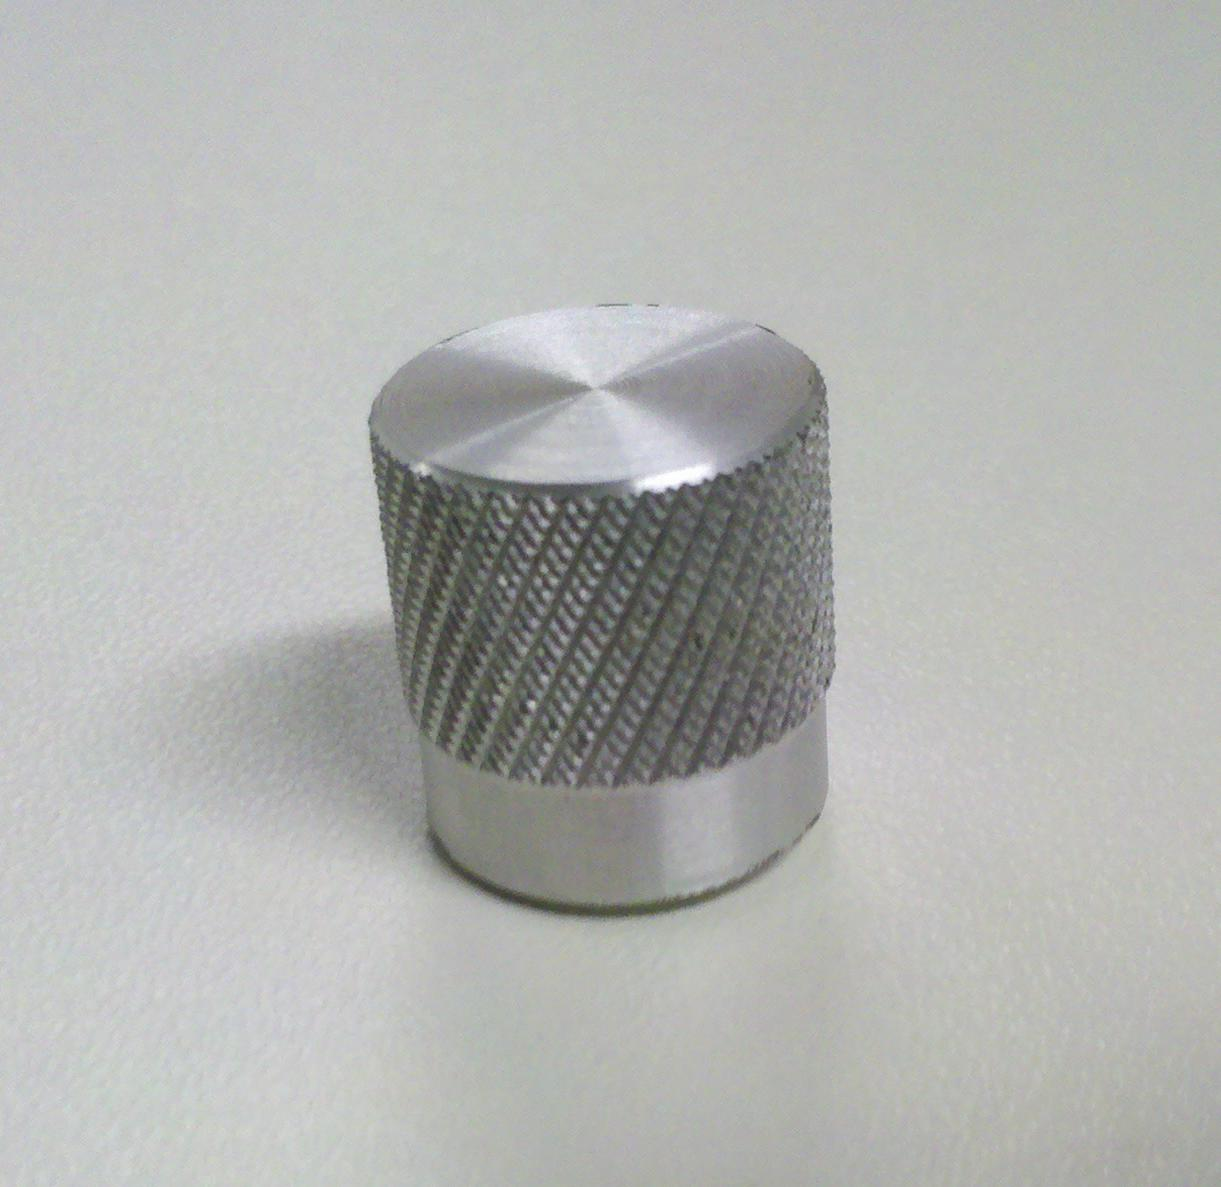
\includegraphics[width=.5\linewidth]{img/raendel}
\end{figure}
\newpage
\section{CNC - Drehen}

\newpage
\section{Aufräumen und Wartung}




\end{document}